% !TEX root = ../Hamiltonian_of_mean_force.tex
\section{Spin-Boson Model}
\label{subsec:qubit_exact_geometry}

The spin-boson model~\cite{leggettDynamicsDissipativeTwostate1987,weissQuantumDissipativeSystems2012} - a two-level system coupled linearly to a
bosonic bath - occupies a unique position in the theory of open quantum systems. It is the simplest
model that captures the full competition between quantum coherence and environmental dissipation, and
it arises as a controlled description across condensed matter, quantum optics, and quantum chemistry,
from Josephson junctions and impurity problems to photosynthetic energy transfer and qubit
decoherence. Despite more than four decades of investigation using path integrals, renormalisation
group methods, numerical renormalisation group, and tensor-network approaches, a general closed-form
solution for the reduced equilibrium state at arbitrary coupling and temperature remains
unknown~\cite{leggettDynamicsDissipativeTwostate1987,weissQuantumDissipativeSystems2012,Bulla2008,Vojta2006}. Exact results are confined to
special limits: weak coupling (Redfield/Born--Markov), the scaling limit near the
Toulouse point, and the zero-temperature ground state in certain parameter regimes. The exact
thermodynamics of the intermediate-coupling, finite-temperature regime remains inaccessible to
standard perturbative techniques. 

In some sense this is an embarrassment for the field. Regardless of whether one marks the model's inception in the 1960s with the Kondo model \cite{Kondo1964}, or its formal coining in the 1980s \cite{leggettDynamicsDissipativeTwostate1987}, it is a problem that has remained open for decades. It is high time for the case to be closed. To do so, we now derive the exact solution for the reduced equilibrium state of the spin-boson model, with the caveat that we deal only with finite temperature. While the necessary machinery for the $\beta \to \infty$ ground state solution is implicit in the present work, we defer its full treatment to future work.

Let us first set our conventions. As in Sec.~\ref{subsec:kms_symmetry}, we work in the qubit energy basis
(\(\hat{\mathbf n}_s=\hat{\mathbf z}\)) during derivation, then state the final geometry in the
coupling plane spanned by \(\hat{\mathbf n}_s\) and \(\hat{\mathbf f}\). We take
\begin{equation}
    H_Q = \frac{\omega_q}{2}\,\hat{\mathbf n}_s\!\cdot\!\boldsymbol{\sigma}, \qquad
    f = \hat{\mathbf f}\!\cdot\!\boldsymbol{\sigma},
\end{equation}
with \(\hat{\mathbf f}=(s\cos\phi,s\sin\phi,c)\), \(c\equiv\cos\theta\), \(s\equiv\sin\theta\).
The dimensionless coupling amplitude \(g\) is suppressed in intermediate expressions and reinserted
where scaling is discussed.

\begin{figure}[t]
    \centering
    
\includegraphics[width=\columnwidth]{../figures/hmf_bloch_3d_overview.pdf}
    \caption{Bloch-sphere geometry with the three radii used in the text.
    The bare thermal state has radius \(r_0\) (blue), the symmetrised influence state
    \(\rho_S\propto e^S\) has radius \(r_S\) and signed tilt \(\varphi_S\) (purple), and the final
    reduced state has radius \(r_Q\) and tilt \(\varphi_Q\) (red). The black arc marks the relative
    rotation \(\Delta\varphi=\varphi_Q-\varphi_S\).}
    \label{fig:bloch_overview}
\end{figure}

\subsection{Bath kernels and the symmetrised influence state}
\label{subsec:qubit_v3_influence_state}

The interaction-picture coupling operator is
\begin{equation}
    \tilde f(\tau)=e^{\tau H_Q}fe^{-\tau H_Q}
    = c\sigma_z + f_-e^{\omega_q\tau}\sigma_+ + f_+e^{-\omega_q\tau}\sigma_-,
\end{equation}
with \(f_\pm=s e^{\pm i\phi}\). The required \(SU(2)\) algebra is standard and relegated to
App.~\ref{app:qubit_ladder_derivation}. The final result is that all bath dependence enters through
two real response channels
\begin{equation}
    \begin{aligned}
    \Sigma_z &\equiv \frac{1}{2}\!\left[R(\omega_q)-R(-\omega_q)\right], \\
    \Sigma_\perp &\equiv \frac{4}{\omega_q}\!\left[
        \cosh\!\left(\frac{\beta\omega_q}{2}\right)\mathcal K(0)
        -e^{-\beta\omega_q/2}\mathcal K(\omega_q)\right].
    \end{aligned}
    \label{eq:bath_kernels_direct}
\end{equation}

Using the symmetric decomposition
\(\bar\rho_Q=\Pi^{1/2}e^S\Pi^{1/2}\), \(\Pi=e^{-\beta H_Q}\), the symmetrised influence operator is
\begin{equation}
    S=\Delta_0\mathbb I
    +s^2\Sigma_z\,\sigma_z
    -sc\,\Sigma_\perp(\cos\phi\,\sigma_x+\sin\phi\,\sigma_y).
    \label{eq:S_symmetrised_v3}
\end{equation}
The influence operator can then be written as \(M\equiv S-\Delta_0\mathbb I = \mathbf m_S\!\cdot\!\boldsymbol{\sigma}\).After some squinting, one sees that its may be written in terms of the perpendicular to the coupling vector, i.e. $\hat{\mathbf f}_\perp = (-c\cos\phi,\,-c\sin\phi,\,s)$. So the influence Bloch vector is
\begin{equation}
    \mathbf m_S=
    s\Sigma_\perp\hat{\mathbf f}_\perp + s^2(\Sigma_z-\Sigma_\perp)\hat{\mathbf n}_s,
    \label{eq:mS_decomposition}
\end{equation}
 The \emph{influence magnitude} is then
\begin{equation}
    \chi=\|\mathbf m_S\|
    =|s|\sqrt{c^2\Sigma_\perp^2+s^2\Sigma_z^2}
    \label{eq:chi_factored}
\end{equation}
note that the magnitude depends on the \emph{absolute value} of $s=\sin\theta$. Unless otherwise stated, all results shall assume $s>0$.

The \emph{influence state} is now naturally given by $\rho_S = \rm{e}^S/\Tr(\rm{e}^S)$. Evaluating this yields
\begin{equation}
    \rho_S=\frac{1}{2}\!\left[\mathbb I+\tanh\chi\,\hat{\mathbf m}_S\!\cdot\!\boldsymbol{\sigma}\right],
    \qquad
    \hat{\mathbf m}_S=\mathbf m_S/\chi.
    \label{eq:expS_closed}
\end{equation}
In this form, the geometry of the influence state on the Bloch sphere is clear. It has radius $r_S$
\begin{equation}
    r_S = \tanh\chi
\end{equation} 
while its angular content in the plane is determined by the bath. The component perpendicular to the coupling vector is set by the transverse (off-resonant) response, while the parallel component is set by the anisotropy between the longitudinal (resonant) and transverse responses. In the isotropic kernel limit \(\Sigma_\perp=\Sigma_z\), that parallel piece vanishes and \(e^S\) points exactly perpendicular to \(\hat{\mathbf f}\). The bath anisotropy is directly encoded in the \emph{signed tilt} of $\rho_S$ from the bare axis (\(-\hat{\mathbf n}_s\)) via the relation
\begin{equation}
    \tan\varphi_S=-\,\frac{c}{s}\,\frac{\Sigma_\perp}{\Sigma_z}.
    \label{eq:phiS_def}
\end{equation}
The sign of \(\chi\propto s\) carries orientability: \((\chi,\hat{\mathbf m}_S)\) and
\((-\chi,-\hat{\mathbf m}_S)\) are equivalent charts of the same physical \(\rho_S\). This discrete
orientability is benign at the \(\rho_S\) stage but becomes consequential after recombination with the
bare Gibbs factor.

\subsection{Reduced state in signed Bloch form}
\label{subsec:qubit_v3_reduced_state}
With \(\rho_S\) in hand, the reduced state follows by recombination with the bare Gibbs factor,
\(\rho_Q = \Pi^{1/2}\rho_S\Pi^{1/2}\). It takes the same Bloch form,
\begin{equation}
    \rho_Q = \frac{1}{2}\big[\mathbb I + r_Q \hat{\mathbf m}_Q \cdot \boldsymbol{\sigma}\big],
\end{equation}
where \(r_Q = \sqrt{m_z^2+m_\perp^2}\) and the components are resolved along and perpendicular to the
bare axis via the tilt angle \(\varphi_Q\):
\begin{equation}
    m_z = r_Q\cos\varphi_Q, \qquad m_\perp = r_Q\sin\varphi_Q.
    \label{eq:tilt_angle_def}
\end{equation}
We can define the effective longitudinal scale by the projection of the influence state onto the bare axis. Defining the factor
\begin{equation}
    \gamma(\chi)\equiv\tanh\chi/\chi
\end{equation}
the effective longitudinal scale is given by
\begin{equation}
    \Theta \equiv \operatorname{arctanh}\!\big(\gamma(\chi)\,s^2\Sigma_z\big)-\frac{\beta\omega_q}{2}.
    \label{eq:theta_param}
\end{equation}
The explicit solution is then
\begin{align}
    m_z &= \tanh\Theta, \label{eq:m_z_solution}\\
    m_\perp &= \tan\varphi_S\!\left(
        m_z\cosh\frac{\beta\omega_q}{2}
        +\sinh\frac{\beta\omega_q}{2}\right),
    \label{eq:bloch_locking_linear}
\end{align}
where \(\varphi_S\) is the tilt angle of the influence state, Eq.~\eqref{eq:phiS_def}.
The structure is clear: \(m_z\) is a thermal magnetisation evaluated at an
\emph{effective} longitudinal scale \(\Theta\), which encodes the bath-renormalised temperature, while
\(m_\perp\) is locked to \(m_z\) through the bath-induced tilt \(\varphi_S\). Defining the bare
system radius as \(r_0=\tanh(\beta\omega_q/2)\), the final tilt angle is
\begin{equation}
    \tan\varphi_Q = \tan\varphi_S\,\frac{m_z + r_0}{\sqrt{1-r_0^2}\;m_z},
    \label{eq:phiQ_def}
\end{equation}
and the radius satisfies
\begin{equation}
    1 - r_Q^2 = \frac{(1-r_0^2)(1-r_S^2)}{(1+r_0 r_S\cos\varphi_S)^2}.
    \label{eq:rQ_geometric_composition}
\end{equation}
Thus recombination acts as a \emph{two-step deformation} of \(\rho_S\): a shift in radius governed
by the competition between \(r_0\) and \(r_S\), controlled ultimately by the influence magnitude and a rotation of the tilt angle from  (definitionally) to \(\varphi_Q\). These effects are ultimately controlled by just three factors - the angle of the coupling, the anisotropy of the bath response, and its effective magnitude \(\chi\).

\section{Thermal renormalisability, duality, and relativity}
\label{subsec:qubit_v3_theta_duality}

The influence state \(\rho_S\) enjoys a discrete orientability symmetry: as noted above, the pair
\((\chi,\hat{\mathbf{m}}_S)\) and \((-\chi,-\hat{\mathbf{m}}_S)\) are equivalent charts of the
same physical state. At the level of \(\rho_S\) this is entirely benign — both charts represent
the same point on the Bloch sphere. After recombination with the bare Gibbs weight, however, this
symmetry is \emph{broken}. The bare factor \(\Pi^{1/2}\) carries a definite orientation along
\(-\hat{\mathbf{n}}_s\), and the two orientability charts of \(\rho_S\) couple to it differently.
The result is a genuine \emph{representational duality} in the reduced state: two inequivalent
thermal descriptions of the same physics.

To expose this duality it is useful to recast the result as a thermal renormalisation. Working in
the bare-system orientation, we observe that the longitudinal component \(m_z = \tanh\Theta\) has
exactly the form of a thermal magnetisation. This motivates defining a \emph{renormalised inverse
temperature}
\begin{equation}
    \bar\beta \equiv -\frac{2\Theta}{\omega_q},
    \label{eq:bar_beta_def}
\end{equation}
so that \(m_z = \tanh(-\bar\beta\,\omega_q/2)\), with corresponding renormalised radius
\(\bar r \equiv |m_z|\). The bath's longitudinal influence then acts as a pure shift of the inverse
temperature from the bare \(\beta\) to
\begin{equation}
    \bar\beta = \beta - \frac{2}{\omega_q}\operatorname{arctanh}\!\big(\gamma(\chi)\,s^2\Sigma_z\big).
    \label{eq:bar_beta_explicit}
\end{equation}
The transverse bath response captures the remainder of the influence by tilting the renormalised
state. This renormalised tilt angle is definitionally equivalent to the reduced state's tilt: \(\bar\varphi = \varphi_Q\). This raises an immediate question: why bother with the relabelling? The answer is that the physical
content depends critically on the \emph{sign} of \(\Theta\), and this is precisely where the
broken orientability of the influence state reasserts itself. 


The two physically transparent special cases illustrate the structure cleanly. For \emph{pure
longitudinal coupling} (\(s=0\)), the influence state is maximally mixed (\(\chi=0\),
\(\rho_S=\mathbb I/2\)), recombination reproduces the bare Gibbs state, and both dual charts
collapse to \(\bar\beta = \beta\): this is the self-dual fixed point with no thermal renormalisation.
For \emph{pure transverse coupling} (\(\theta=\pi/2\), \(c=0\)), the longitudinal response
vanishes identically (\(\Sigma_z\mapsto0\)), the tilt angle \(\varphi_Q\to 0\), and the
renormalised temperature reduces to
\begin{equation}
    \bar\beta\big|_{\Sigma_z=0} = \beta \pm \frac{2\Sigma_\perp}{\omega_q},
    \label{eq:bar_beta_transverse}
\end{equation}
where the two signs correspond to the two dual charts. A purely transverse coupling is therefore
nothing more than a shift in effective temperature, with the direction of the shift set by the
relative orientation of coupling and bare-system axis.

The key observation is that the operation \(\theta\mapsto\pi-\theta\) (i.e.\ reflecting the
coupling vector about the equatorial plane, \(c\to-c\), \(s\to s\)) admits two complementary
readings. From the geometric side, it is a \emph{global phase}: since \(\chi\propto|s|\), the
influence radius \(r_S=\tanh\chi\) is invariant, and the operation is simply a relabelling of the
coupling orientation that leaves \(\rho_S\) unchanged. But to maintain exactly the same influence
state \(\rho_S\) when passing from \(\theta\) to \(\pi-\theta\), the bath must compensate: its
longitudinal susceptibility must undergo \(\Sigma_z\mapsto-\Sigma_z\). In this second reading, the
same discrete transformation is a genuine \emph{symmetry-breaking operation} — a change in the
bath susceptibilities, not a geometric relabelling. The duality between the two reduced-state
representatives is the footprint of this ambiguity: the influence state \(\rho_S\) cannot
distinguish the two, but after recombination with the bare Gibbs weight, \(\rho_Q\) can.
Under \(\Sigma_z\mapsto-\Sigma_z\) at fixed \(\theta\), the effect on the longitudinal scale is
$\operatorname{arctanh}(\gamma s^2 \Sigma_z) \mapsto -\operatorname{arctanh}(\gamma s^2 \Sigma_z)$, giving
\begin{equation}
    \Theta \;\mapsto\; -\Theta - \beta\omega_q, \qquad
    \bar\beta \;\mapsto\; 2\beta - \bar\beta, \qquad
    \varphi_Q \;\mapsto\; \pi - \varphi_Q.
    \label{eq:orientation_flip}
\end{equation}
The two reduced states are genuinely distinct - a reflected tilt and a dual temperature - but are possess a natural \emph{duality} structure. At the level of \(\bar\beta\), we have the dual charts:

\begin{equation}
    \bar\beta^{\,\vee} = 2\beta - \bar\beta,
    \qquad
    \bar\beta + \bar\beta^{\,\vee} = 2\beta,
    \label{eq:beta_eff_duality}
\end{equation}
with \(\bar\beta = \beta\) (i.e.\ \(\Theta = 0\)) as the self-dual symmetry
point. One orientability chart renormalises the temperature upward; the other renormalises it
downward. The dual mappings for the renormalised radius and tilt angle take the equally compact forms
\begin{equation}
    \operatorname{arctanh}\bar r + \operatorname{arctanh}\bar r^{\,\vee} = \beta\omega_q,
    \qquad
    \varphi_Q + \varphi_Q^{\,\vee} = \pi,
    \label{eq:dual_radius_angle}
\end{equation}
mirroring the structure of Eq.~\eqref{eq:beta_eff_duality}: the dual pairs each sum to their
natural full-scale value (\(2\beta\), \(\beta\omega_q\), and \(\pi\) respectively).
Since \(\operatorname{arctanh}r = \frac{1}{2}\ln\frac{1+r}{1-r}\), the radius relation is
equivalently a constraint on the product of polarisation ratios,
\begin{equation}
    \frac{1+\bar r}{1-\bar r}\cdot\frac{1+\bar r^{\,\vee}}{1-\bar r^{\,\vee}}
    =\left(\frac{1+r_0}{1-r_0}\right)^{\!2},
    \label{eq:dual_radius_multiplicative}
\end{equation}
making the opposite-scaling property explicit: if \(\bar r > r_0\) (temperature renormalised
downward), then necessarily \(\bar r^{\,\vee} < r_0\) (renormalised upward), and vice versa.
The structure is manifestly relativistic: identifying \(\operatorname{arctanh}\bar r\) with a
rapidity, the dual constraint is a fixed sum of rapidities — precisely the kinematics of a Lorentz
boost, with the bare Gibbs factor playing the role of the boost. The iso-dual curves are
rectangular hyperbolas (cf.\ the dual-pair lines in
Fig.~\ref{fig:minkowski_diagram}). All three dual maps are \emph{involutive} — applying either
map twice returns the original value — with the common self-dual fixed point at
\(\bar\beta=\beta\), \(\bar r = r_0\), \(\varphi_Q=\pi/2\).

The tilt angle offers a complementary picture. Defining the centred deviation
\(\psi\equiv\varphi_Q-\pi/2\), the dual map simply sends \(\psi\mapsto -\psi\): the two
representations sit at equal and opposite angles about the self-dual point. This motivates a final interpretation of the duality structure created by the bath symmetry breaking. In the relativistic language, the rapidity (radius) and tilt (angle) play conjugate roles — the rapidities sum to a positive constant (timelike), while the centred tilts are equal and opposite (spacelike). Together they equip the dual structure with the signature of a Minkowski metric, with the self-dual fixed
point at its light-cone vertex. Using \(\eta\equiv\operatorname{arctanh}\bar r = \bar\beta\omega_q/2\)
and centred coordinates \(\delta\bar\beta\equiv\bar\beta-\beta\), \(\psi\equiv\varphi_Q-\pi/2\),
the flat metric and its preserved interval take the explicit form
\begin{equation}
    ds^2 = \left(\frac{\omega_q}{2}\right)^{\!2}d\bar\beta^{\,2} - d\varphi_Q^2,
    \qquad
    s^2 = \left(\frac{\omega_q\,\delta\bar\beta}{2}\right)^{\!2} - \psi^2,
    \label{eq:minkowski_metric}
\end{equation}
with the dual map acting as the point reflection \((\delta\bar\beta,\psi)\mapsto(-\delta\bar\beta,-\psi)\)
about the origin. States with \(s^2>0\) are ``timelike'': temperature renormalisation dominates;
states with \(s^2<0\) are ``spacelike'': the tilt dominates. The light cone
\(|\omega_q\delta\bar\beta/2|=|\psi|\) divides these regimes and passes through the self-dual
fixed point.



\begin{figure}[t]
    \centering
    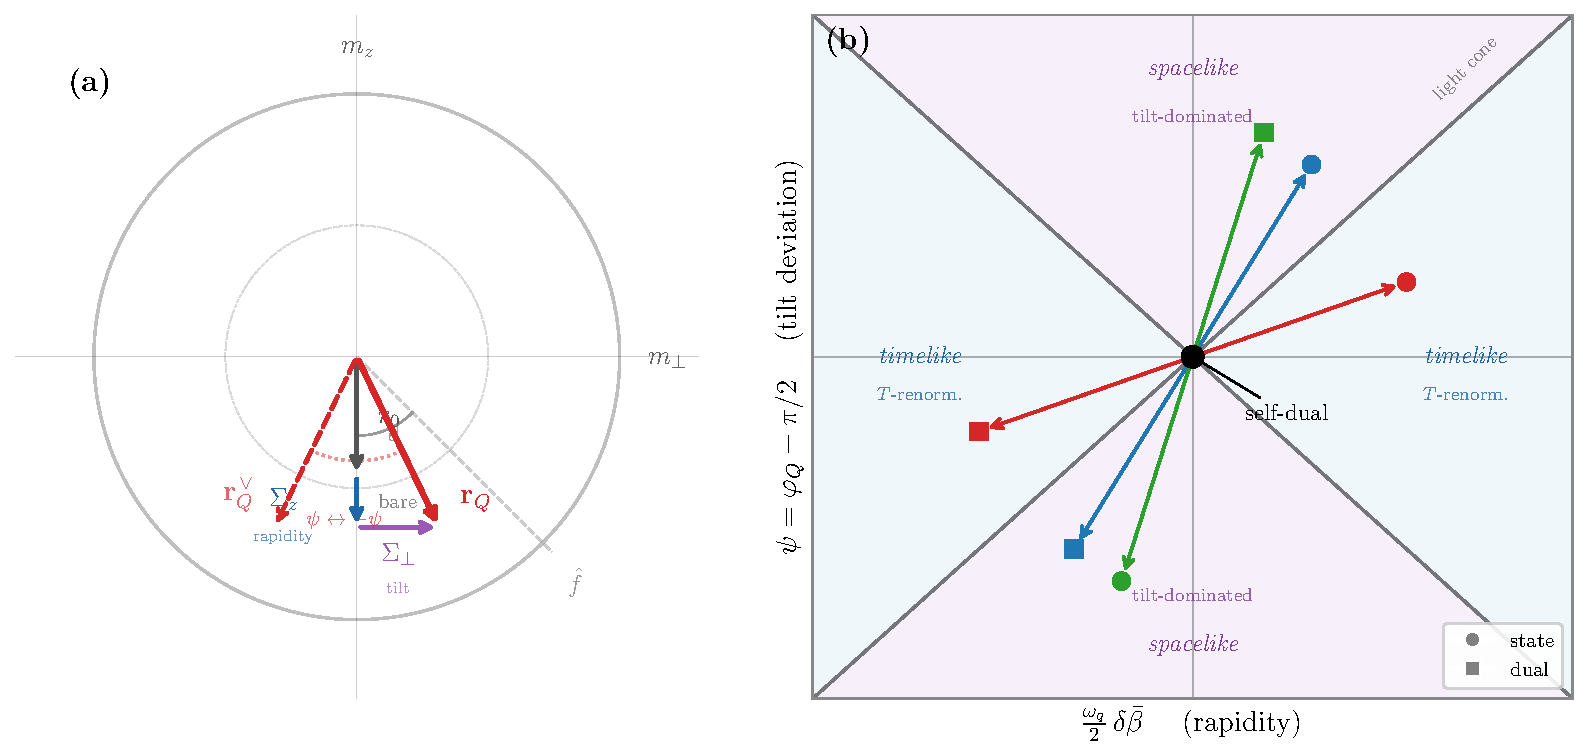
\includegraphics[width=\columnwidth]{../figures/hmf_minkowski_hero.pdf}
    \caption{Thermodynamic Minkowski diagram in the centred thermal
    coordinates $(\omega_q\delta\bar\beta/2,\,\psi)$
    (Eq.~\eqref{eq:minkowski_metric}). The dual map acts as a point
    reflection about the self-dual origin ($\bullet$), exchanging each
    state (circles) with its dual (squares). Temperature renormalisation
    dominates in the timelike (blue) sectors; tilt dominates in the
    spacelike (purple) sectors.}
    \label{fig:minkowski_diagram}
\end{figure}

It feels somewhat glib to observe a rectangular hyperbola and immediately declare a relativistic
structure, but in the present case it is difficult to avoid. The thermodynamic description of black holes has been long established, and the present argument simply repays the favour from the opposite orientation. In this language the role of \emph{mass} is played by

the bare transition frequency \(\omega_q\): it is the single scale of the two-level spectrum, and
it sets the ``speed'' of the timelike coordinate in Eq.~\eqref{eq:minkowski_metric}. Different
values of \(\omega_q\) correspond to different families of hyperbolas — different mass shells.

The generalisation to an \(N\)-level system is immediate in spirit, though with an important
refinement: there is still only \emph{one} physical temperature \(\beta\). The \(K=N(N-1)/2\)
transition frequencies \(\{\omega_k\}\) each carry their own renormalised inverse temperature
\(\bar\beta_k(\beta)\), but these are not independent — they all descend from \(\beta\) through
the bath's sector-specific renormalisations. Defining the \emph{thermal renormalisation tensor}
\begin{equation}
    \mathcal{T}_k \equiv \frac{\partial\bar\beta_k}{\partial\beta},
    \label{eq:thermal_T_tensor}
\end{equation}
the physical metric lives on the image of the map \(\beta\mapsto\{\bar\beta_k(\beta)\}\). The
timelike sector collapses back to a single coordinate \(\beta\), dressed by \(\mathcal{T}\):
\begin{equation}
    ds^2 = \left[\sum_k \left(\frac{\omega_k}{2}\right)^{\!2} \mathcal{T}_k^{\,2}\right] d\beta^2
    - \sum_k d\psi_k^2.
    \label{eq:metric_N_level}
\end{equation}
The bracketed coefficient — a weighted sum of squared renormalisation Jacobians — is the
\(N\)-level generalisation of \((\omega_q/2)^2\) and constitutes the stress-energy content: the
spectrum \(\{\omega_k\}\) sets the mass scale of each sector, while \(\mathcal{T}_k\) encodes
how strongly the bath couples each transition to the physical temperature. The
bath-induced angles \(\psi_k = \varphi_{Q,k}-\pi/2\) supply the spacelike (momentum) content. A
purely longitudinal coupling concentrates the ``matter'' on the timelike axis; general couplings
distribute it across the light cone. The transition to a general-relativistic language is the
passage to systems where the \(\mathcal{T}_k\) vary across parameter space — precisely many-body
or multi-mode environments where the coupling geometry itself becomes state-dependent. Amusingly, this apparent linearisation of the relativistic field theory is a natural consequence of the one \emph{nonlinear} operation in quantum theory. The trace.  A formal proof of this mapping is left as an exercise to the reader. We expect this to lie within the capacities of even the least creatively burdened physicist. 



